\chapter{Implementation}
\label{chapter3}

This chapter will go through the implementation of the project. First, the system information and general program structure will be looked at. Then, the rendering of fractals will be covered, followed by the attempts at improving performance, and the method of measuring performance. Finally, there will be a section on debugging.\newline

In terms of general optimizations, there were no specific efforts to optimize the code or the basic algorithms (except perhaps to implement a view distance limit), since the most important thing was to remain consistent across the different scenarios, and the relevant measurements were the performance differences (if any), not the raw performance.

\section{Operating System and Hardware}

The operating system used was Linux Mint 20.1. The project compiles on Linux using Make. Considering that the project was written in C, it is likely very portable (as long as the system can use Vulkan as well), but compilation on other operating systems has not been tested, and may require changes to the method of compilation.\newline

The CPU used was an Intel\copyright Core$^{TM}$ i7-9750H with 6 cores.

The GPU used was an NVIDIA TU106M (GeForce RTX 2060 Mobile).

The Vulkan version being used was 1.3.205.

\section{Program Structure and Libraries}

\subsection{Language and Libraries Used}

The programming language of choice for this project was C, because it is the language that the libraries used were written in, and it's simple and efficient.

\subsubsection{Vulkan}

Vulkan was chosen because it is performant and modern, and because there is a new feature on the way that will, I think, help with the efficiency of rendering using one of the optimization methods chosen (this will be mentioned in the Conclusion chapter). It is licensed under the Apache License 2.0 \cite{licensing-vulkan}.

\subsubsection{Volk}

The third-party library, Volk, is a meta-loader for Vulkan. It allows one to load the Vulkan API without needing to link to Vulkan. This makes setup much easier to manage. It is licensed under the MIT license \cite{licensing-volk}.

\subsubsection{GLFW}

GLFW is a library for creating windows and surfaces, which can be used for Vulkan development. Additionally, it is easy to use and multi-platform, so was the logical choice for this project. It is licensed under the zlib/libpng license \cite{licensing-glfw}.

\subsection{Vulkan Setup}

The rendering process was split into two passes, one for geometry and one for colour. This was done because the speed at which the geometry of the scene was obtained was of interest, and the speed of colouring the fractals was not, so splitting them enabled measurement of the geometry render pass on its own. No vertices are passed in to the shaders; the vertex shaders conjure up fullscreen triangles using the vertex indices, which are then worked on by the fragment shaders, where all the calculations and colouring happen.\newline

Specific setups for different optimization methods will be discussed in the relevant sections.

\subsection{Program Arguments and Controls}

The program takes arguments which specify the setup when the program is loaded. The user can change which fractal to display (including the 2D Mandelbrot set, the Mandelbulb and the Hall of Pillars), which optimization method to use, whether to vary any fractal parameters (which can be used to animate the fractal) and whether to take any performance measurements during runtime. Some of the arguments affect which shaders are loaded, and the Vulkan setup.\newline

The user is able to control the camera with the mouse and keyboard, speed up and slow down, and print the current position and camera front vector. Input is handled by GLFW.

\section{Rendering 3D Fractals}

The project made use of two fractal formulae. One was for the Mandelbulb, as described in the background section. Another was chosen to provide variety, specifically with regards to the depth of the image. The Mandelbulb is neatly contained within a box, and the program renders its exterior, but not any `interior'. The alternative fractal (named `Hall of Pillars' by me given its lack of another name) is reminiscent of a room with many archways, which I thought might give a greater variety of results in terms of the performance measurements when using the optimizations developed in the project.\newline

The calculations for the fractals were done entirely within shaders, except for the generation of the 3D signed distance field, which was calculated on the CPU upon loading the program, before any rendering occurred. Single-precision floating point numbers were used for all calculations within shaders. These were chosen over double-precision numbers, as the scale of the fractals was reasonable, and high-detail zooms into the fractal were not necessary for the project.

\subsection{Basic Sphere Tracing Implementation}

The basic sphere tracing algorithm was implemented in GLSL and is largely the same across the fractal types and optimization methods. Figure \ref{figure:glsl-sphere-tracing} shows the implementation.

\begin{figure}[ht]
	\centering
	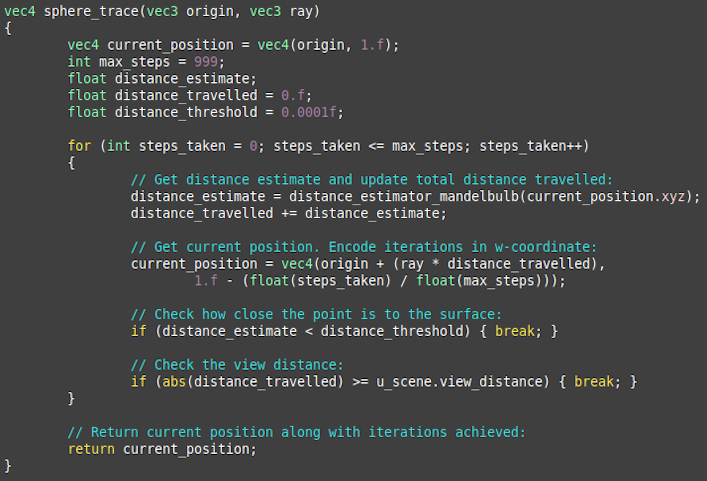
\includegraphics[width=0.65\linewidth, frame]{Images/GLSL-Sphere-Tracing.png}
	\caption{GLSL code snippet of the sphere tracing algorithm.}
	\label{figure:glsl-sphere-tracing}
\end{figure}

The most important things that must remain consistent between different optimizations on the same fractal are the termination conditions, which are as follows:

\begin{itemize}
	\item The maximum number of iterations allowed.
	\item The distance threshold.
	\item The view distance, contained in the scene uniform.
\end{itemize}

\subsection{Mandelbulb Fractal}

\begin{figure}[ht]
	\centering
	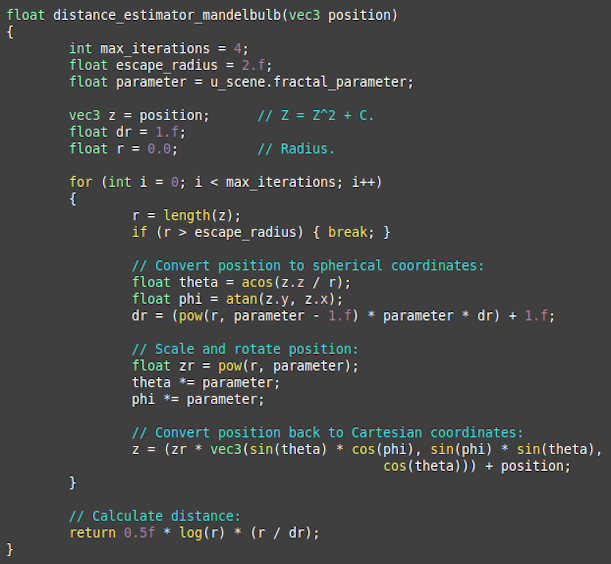
\includegraphics[width=0.65\linewidth, frame]{Images/GLSL-Distance-Estimator-Mandelbulb.png}
	\caption{GLSL code snippet of the distance estimator function for the Mandelbulb fractal.}
	\label{figure:glsl-distance-estimator-mandelbulb}
\end{figure}

\begin{figure}[ht]
	\centering
	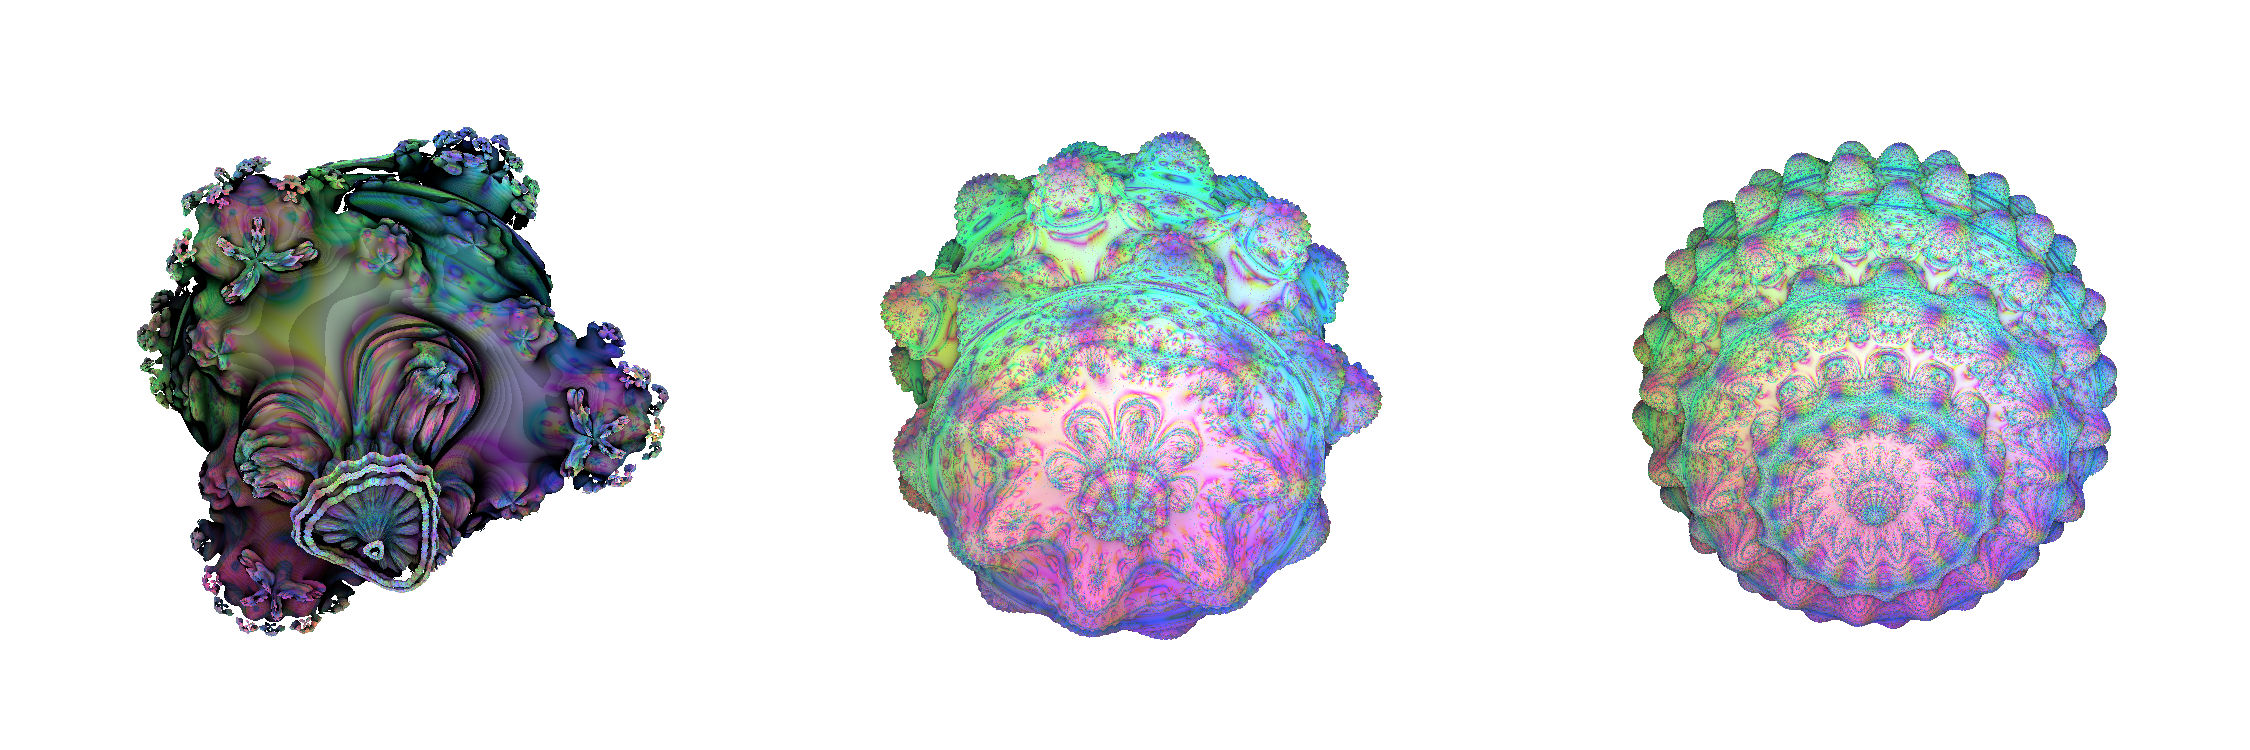
\includegraphics[width=0.65\linewidth, frame]{Images/Mandelbulb-Powers.png}
	\caption{The Mandelbulb, raised to different powers. Left to right: four, eight, sixteen.}
	\label{figure:mandelbulb-powers}
\end{figure}

Figure \ref{figure:glsl-distance-estimator-mandelbulb} shows the implementation of the distance estimator for the Mandelbulb fractal. Recall equations \ref{equation:mandelbulb} and \ref{equation:mandelbulb-power}. Equation \ref{equation:mandelbulb} is iterated over four times maximum. During the iterations, the current point is converted to spherical coordinates, scaled, and then converted back to Cartesian coordinates using equation \ref{equation:mandelbulb-power}. The distance formula based on equation \ref{equation:final-distance-estimate} is used to get the final result. The gradient of |f(Z)| is computed during the iterations (represented by dr in the shader).\newline

The fractal parameter in the scene uniform is the power that Z is raised to in the Mandelbulb formula. Varying this parameter results in different forms of the Mandelbulb. By default this parameter is eight, to match the original discovery by Paul Nylander. Figure \ref{figure:mandelbulb-powers} illustrates the effect of varying this parameter.

\subsection{Alternative Fractal}

\begin{figure}[ht]
	\centering
	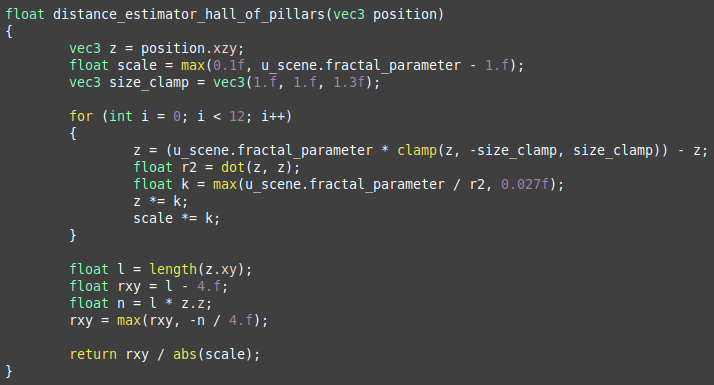
\includegraphics[width=0.65\linewidth, frame]{Images/GLSL-Distance-Estimator-Hall-Of-Pillars.png}
	\caption{GLSL code snippet of the distance estimator function for the Hall of Pillars fractal. Full credit goes to Dave Hoskins for the formula \cite{shadertoy-hall-of-pillars}.}
	\label{figure:glsl-distance-estimator-hall-of-pillars}
\end{figure}

\begin{figure}[ht]
	\centering
	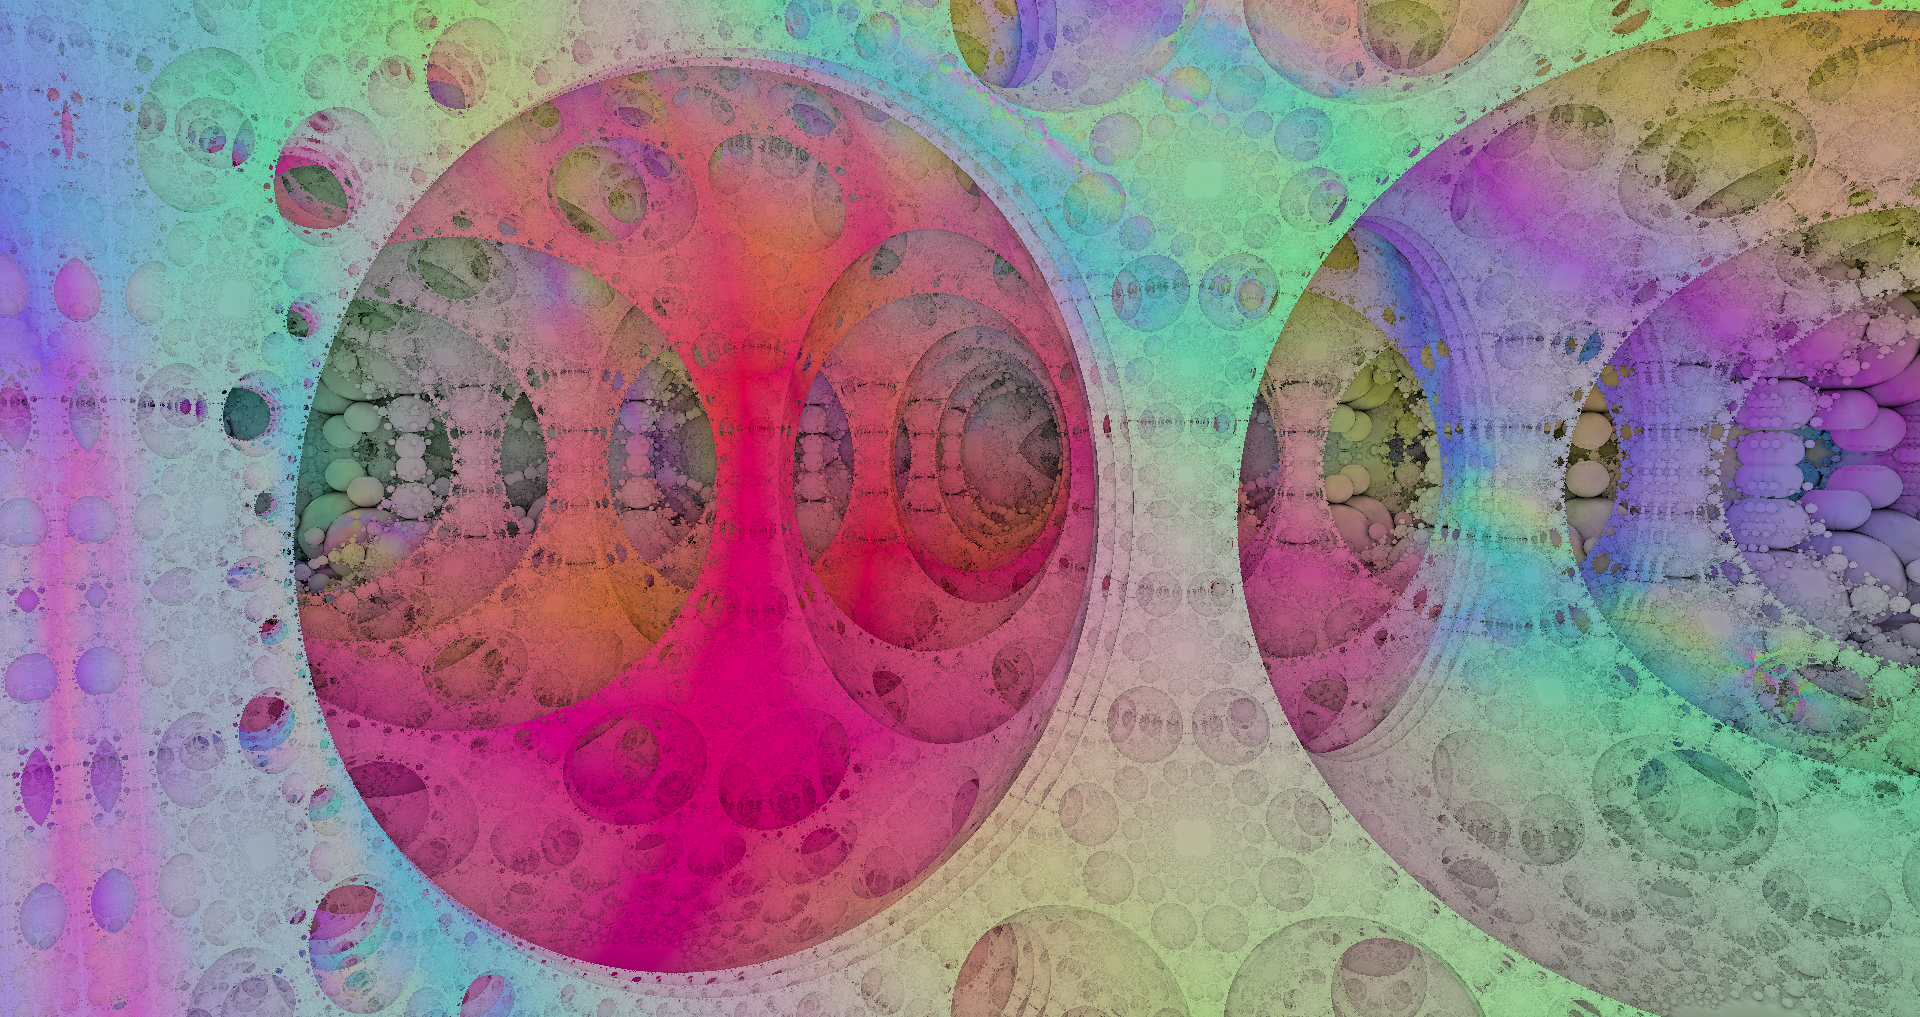
\includegraphics[width=0.65\linewidth, frame]{Images/Hall-Of-Pillars-Example.png}
	\caption{Rendering of the Hall of Pillars fractal.}
	\label{figure:hall-of-pillars-example}
\end{figure}

Figure \ref{figure:glsl-distance-estimator-hall-of-pillars} shows the implementation of the distance estimator for the alternative `Hall of Pillars' fractal. This fractal has different mathematical origins to the Mandelbulb, and is known as a Pseudo Kleinian fractal, but the mathematical background will not be explored here \cite{pseudo-kleinian-fractals}.\newline

As you can see from figure \ref{figure:hall-of-pillars-example}, this fractal varies a lot in depth, and  in particular has a lot of holes in it, so will result in the bottlenecks discussed in section \ref{section:temporal-caching}. The fractal formula was chosen for this reason, and to give variety when collecting results. Exploring the fractal also reveals large flat sections, and even larger `halls' much like the one in figure \ref{figure:hall-of-pillars-example}, as well as more intricate sections with great depth variety, but less overall depth. This fractal provided a good set of representative views for results collection.

\subsection{Colour}

Colour was not of the utmost importance in the project, so this section will be very brief. Colouring of the mandelbulb was done based on the closest distance from each point in the image to some fixed point. The Mandelbulb equation was iterated through, as in the distance estimation function, but in each iteration, the distance of the current point to a fixed point was measured, and the minimum of these was taken as a colour value.\newline

For the Hall of Pillars fractal, the colour was obtained in each iteration by getting the difference between elements of the current point and the previous point, and accumulating these differences.

\subsection{Ambient Occlusion}

\begin{figure}[ht]
	\centering
	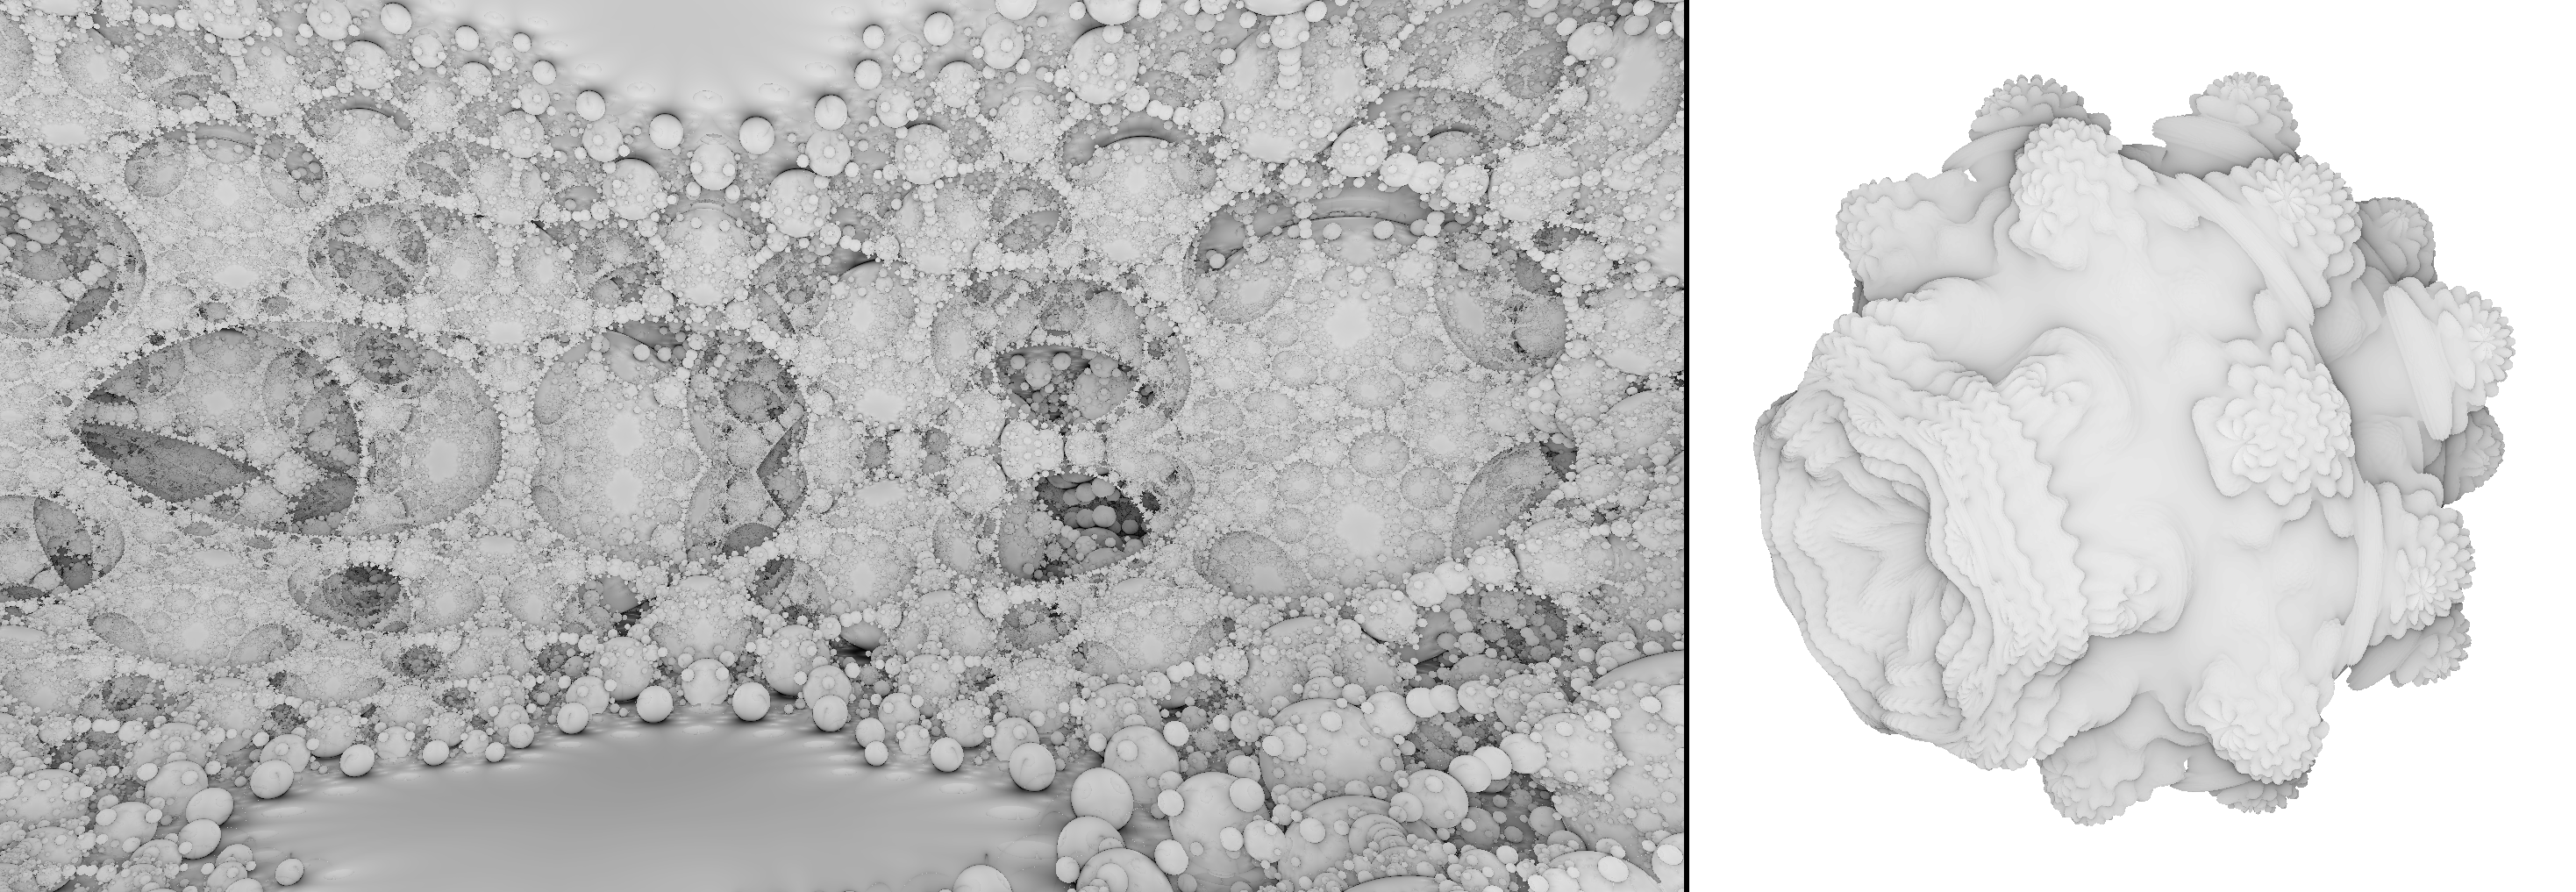
\includegraphics[width=0.65\linewidth, frame]{Images/Ambient-Occlusion.png}
	\caption{Rendering of the Hall of Pillars fractal, coloured based on the number of iterations achieved before reaching the surface.}
	\label{figure:ambient-occlusion}
\end{figure}

One of the consequences of using sphere tracing of signed distance functions is that it gives an estimate of the complexity of the surface. If a point takes more iterations to reach, then it's likely in a more complex area, and will be occluded. For both fractals in the project, the final colour is multiplied by a value between zero and one, based on the number of iterations achieved before reaching the surface. Figure \ref{figure:ambient-occlusion} shows the Hall of Pillars fractal, coloured purely based on the number of iterations.\newline

This free ambient occlusion effect also gives an informal measure of performance. Brighter areas mean less iterations, so two identical views can be compared which are using different optimization methods, to see if one performs better in terms of the number of iterations. Since this was the aim of using temporal caching, this was used as a measure of performance, in addition to render pass timings.

\section{3D Signed Distance Field}

Centered around fractal - Mandelbulb

Centered around camera - Hall of Pillars?

\section{Temporal Caching}

\subsection{Data to Cache}

The data chosen to persist across frames was the true distance travelled by the ray. The aim of this optimization method was to reduce the number of iterations in certain areas of the image, especially edges and holes, so just storing the first distance estimate was not the solution. In order to preserve depth data for multiple frames, a texture image with red, green, blue and alpha floating-point components was chosen. With this, the data for the last four frames was stored.\newline

Alternative data was experimented with as well, such as end position, end distance estimate and the first distance estimate along the ray that was below a certain threshold. The end position was intended to help reveal if the end pixel location had moved too much, invalidating the data. To do this, the stored estimate was used to march the point along the ray for the current frame. The magnitude of the difference between the end position for the last and current frames was then used to determine validity. The end distance estimate was used for the same purpose, but allowed data to be stored for two previous frames, as opposed to just one. The reasoning behind only using one texture image was that sampling a texture requires an overhead that quickly builds up, so storing too much data may offset any performance benefit.\newline

The first distance estimate along the ray was intended to help determine if the current ray was close to an edge. As mentioned in section \ref{section:temporal-caching}, if some geometry occluded the ray, and the distance stored was greater than the distance to that geometry, artefacts would appear. A test was performed that would determine the risk that this had happened, based on the stored distance to an edge.\newline

In the end, storing the true distance travelled for the last four frames worked the best for performance and for artefacts.

\subsection{Camera Movement}

\begin{figure}[ht]
	\centering
	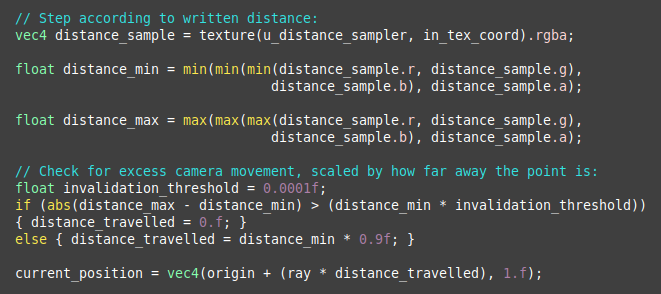
\includegraphics[width=0.65\linewidth, frame]{Images/Distance-Test.png}
	\caption{Test to determine if a pixel is invalid and the ray needs recasting.}
	\label{figure:distance-test}
\end{figure}

The test to see if the camera had moved too much is shown in figure \ref{figure:distance-test}. It relied on the difference between the largest distance sample and the smallest. Generally speaking, the `landscape' of the fractals chosen is not smooth, so this proved to be a reliable test for invalidated geometry, without triggering at the smallest movement. If the test passed, and the pixel was still valid, the minimum sampled distance estimate was chosen and reduced a little, to provide a reliable underestimate of the true distance for the current frame. The usual sphere tracing algorithm was then performed, using this head-start.\newline

The distance values were written to the G-Buffer for the first render pass. Every frame, the values were shifted one place to the right, discarding the last (alpha) value each time, and the new value was written to the first slot. After the render pass, the G-Buffer image was the copied over to a texture image, ready for sampling from during the next frame. Each pixel only sampled from its own position in the texture. It could be possible to do a kind of edge detection based on the depth values in neighbouring pixels, but this was deemed too expensive.

\section{Performance Measurement}

This section will go over how performance differences were measured, and how different scenarios were captured.

\subsection{Data Types Collected}

The main value taken to measure performance was the execution time of the geometry render pass. To accomplish this, a Vulkan query pool was used to collect timestamps at two different stages each frame. One stage was at the beginning of the render pass and one was at the end, in order to make sure the timestamps were taken at the correct times (Vulkan commands in a command buffer may execute in any order unless specific synchronization is added), and consistently, with flags specifying the pipeline stages at which to take the measurements.\newline

Measurements were gathered over a total of one hundred frames before being written out to file. This was to reduce the likelihood of outliers in the data. The minimum, median and maximum values of these sets were taken, as well as the average frame time over the one hundred frames. The median was of the most interest here, as it represents the most likely case, but differences between the other measurements across optimization methods were interesting to look at as well.\newline

The time it took to copy the image after the render pass was not included in the measurements, because copying the image could have been avoided by swapping the G-Buffer image and texture image after the render pass.

\subsection{Representative Views}

Hall of Pillars - Room with archway

Hall of Pillars - Flat ground

Hall of Pillars - Room with huge distance differences and bottlenecks

Hall of Pillars - Room with very short distance to back, maybe bottlenecks

Mandelbulb - Full view, lots of white space

Mandelbulb - Zoomed in so it covers the screen

Mandelbulb - Try to find a view with bottleneck

Mandelbulb - Zoom in to get detail

\subsection{Animation}

Hall of Pillars - Flythrough

Hall of Pillars - Varying parameter?

Mandelbulb - Varying parameter

Mandelbulb - Fly across? Probably not.

\section{Debugging}

Debugging for this project was done manually by printing information out to the terminal. There is a function to print out all values, including handles, for the program's Vulkan structures, to check that they have been initialized properly and to track any Vulkan errors.\newline

To debug the three-dimensional SDF, there is a function to print a subset of the voxels, to check that the search process works properly and that the voxels are stored in the correct order and with the expected range of values.\newline

The key to print the current position and camera front came in useful for checking camera movement, as well as creating animations.\newline

I also used Valgrind to search for and fix any errors with memory management. Unfortunately, it seems that either Vulkan or Volk causes some memory leaks, so debugging this was tricky. I commented out all functions to do with Vulkan (which, admittedly, is most of the program), and there were no leaks or errors. I uncommented only the function that initializes Volk, and it introduced memory leaks.\newline

I debugged the shaders by adding special return values at various locations, so that if there was a problem or a statement was not running when it should have been, the rendered image would not be as expected (for example, it may be entirely black). This was used in combination with RenderDoc to view the different render passes and pipeline stages.